%
\section{Laundry database library}

Most of the project subtask groups decided to use one programming language to make it easier to work together. Sometimes different languages can be difficult connect and operate together. Therefore it was decided to use one object oriented language - C\#. As we know C\# is a one of the new generation languages, which provides a lot of advance features like strong type checking, a garbage collector, robustness and durability. \\ This kind of language makes it easier to develop programs like the subtask, because there is not needed take care of low level features like memory allocation or lost pointer, since low level design is not essential for this subtask. So this kind of language can decrease the duration of the development process and increase code efficiency. \\

All data were stored in MySQL database. Many of subtasks would need access to it and that is why were decided to create a library providing access for any subtask to use. The design requirement is to create a general library which has the features of:  reliability, easy maintenance and simple to use.

\subsection{Design phase}

Due to the mentioned requirements and features it was decided to create a DLL (dynamic link library). The library inside has two classes:

\begin{itemize}
	\item MySQLConnection – database connector which responsible for connection to database and send/receive queries.
	\item Functions – general library for laundry database.
\end{itemize}

\begin{figure}[h]
	\centering
		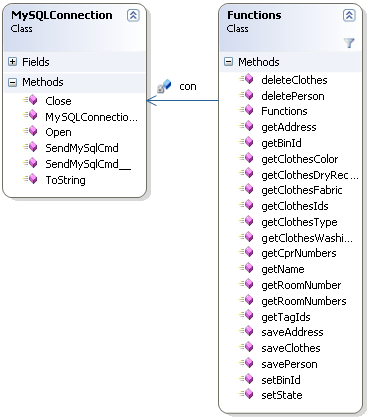
\includegraphics[scale=0.7]{classLibrary}
	\caption{Class library of the database connection}
	\label{fig:planning}
\end{figure}

\newpage
\subsection{Implementation}

Software development was related to unified process (UP) – iterative incremental process.  Iterative incremental process model \cite{bib5} was used during the implementation.  
Let us explain everything in more detail. Project were created using class Library in Microsoft Visual C\# .NET 3.5. To have database connection were included MySQL Connector Net 1.0.10 into references. To use created library we need include it into new project (Console or Win or else) and start our library. For example we insert our library into console project, so connection to database is like shown in the figure 6.1. After successful connection we can use class functions and manage laundry database. 

\begin{figure}[h]
	\centering
		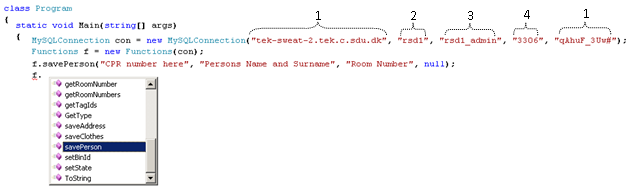
\includegraphics[scale=0.7]{connectionToData}
	\caption{Connection to database server and save new person}
	\label{fig:planning}
\end{figure}

Numbers explain database connection parameters:

\begin{enumerate}
	\item IP address or domain
	\item Database name
	\item User Id
	\item Port number
	\item Password
\end{enumerate}

Class functions uses created instance of MySQLConnection library. And throw the variable f can be connected to all created methods. At the figure 6.2 shows an example of creation new person. As we can see there used methods send queries to database. New CPR inserted into table person by query: “INSERT INTO Person (CPR) Values (‘1234567890’)”.

\begin{figure}[h]
	\centering
		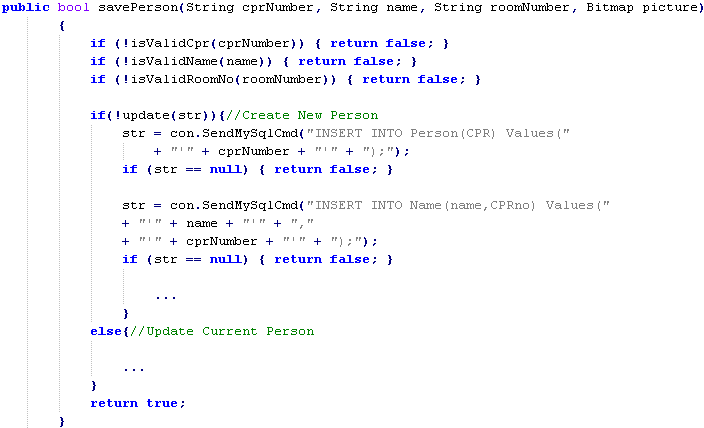
\includegraphics[scale=0.7]{exampleSavePerson}
	\caption{Example of save person method}
	\label{fig:planning}
\end{figure}

\subsection{Future work}